\documentclass{article}
\usepackage{multirow}
\usepackage[inkscapelatex=false]{svg}
\usepackage{amsmath, graphicx}
\usepackage{subfiles}
\usepackage{url}
\usepackage{tabularx}

\title{Git Assignment}
\author{Samuel Olowofila}
\date{}

\begin{document}

\maketitle

\section{Course Goal}
\subsection{Personal Information}
As a 3rd year PhD student in the Bioinformatics, Machine Learning, and Computational Biology research domain, the aforementioned expectations are especially imperative to me. 
I am of Nigerian origin. I am a nerd who enjoys technological innovations in the healthcare and B2B software solutions industries and takes pleasure in actively participating in them. Within the past two years, I have served as a teaching assistant for courses inclusive of Automata and Formal Languages (CS6000), Compiler Design (CS4100), and Computational Thinking with Beginning Programming (CS1120). Currently, I am a graduate research assistant in the UCCS Bioinformatics laboratory under the advisory of Dr. Oluwatosin Oluwadare, the laboratory director.

\begin{figure}[ht!]
    \centering
    \includegraphics[width=0.5\textwidth]{images/sam.png}
    \caption{Samuel at his desk in the UCCS Bioinformatics Lab.}
    \label{Samuel}
\end{figure}

\section{My Research Related GitHub Test}
\begin{itemize}
    \item Repository URL: \url{https://github.com/OluwadareLab/HiCARN.git}
\end{itemize}
\begin{figure}[ht!]
    \centering
    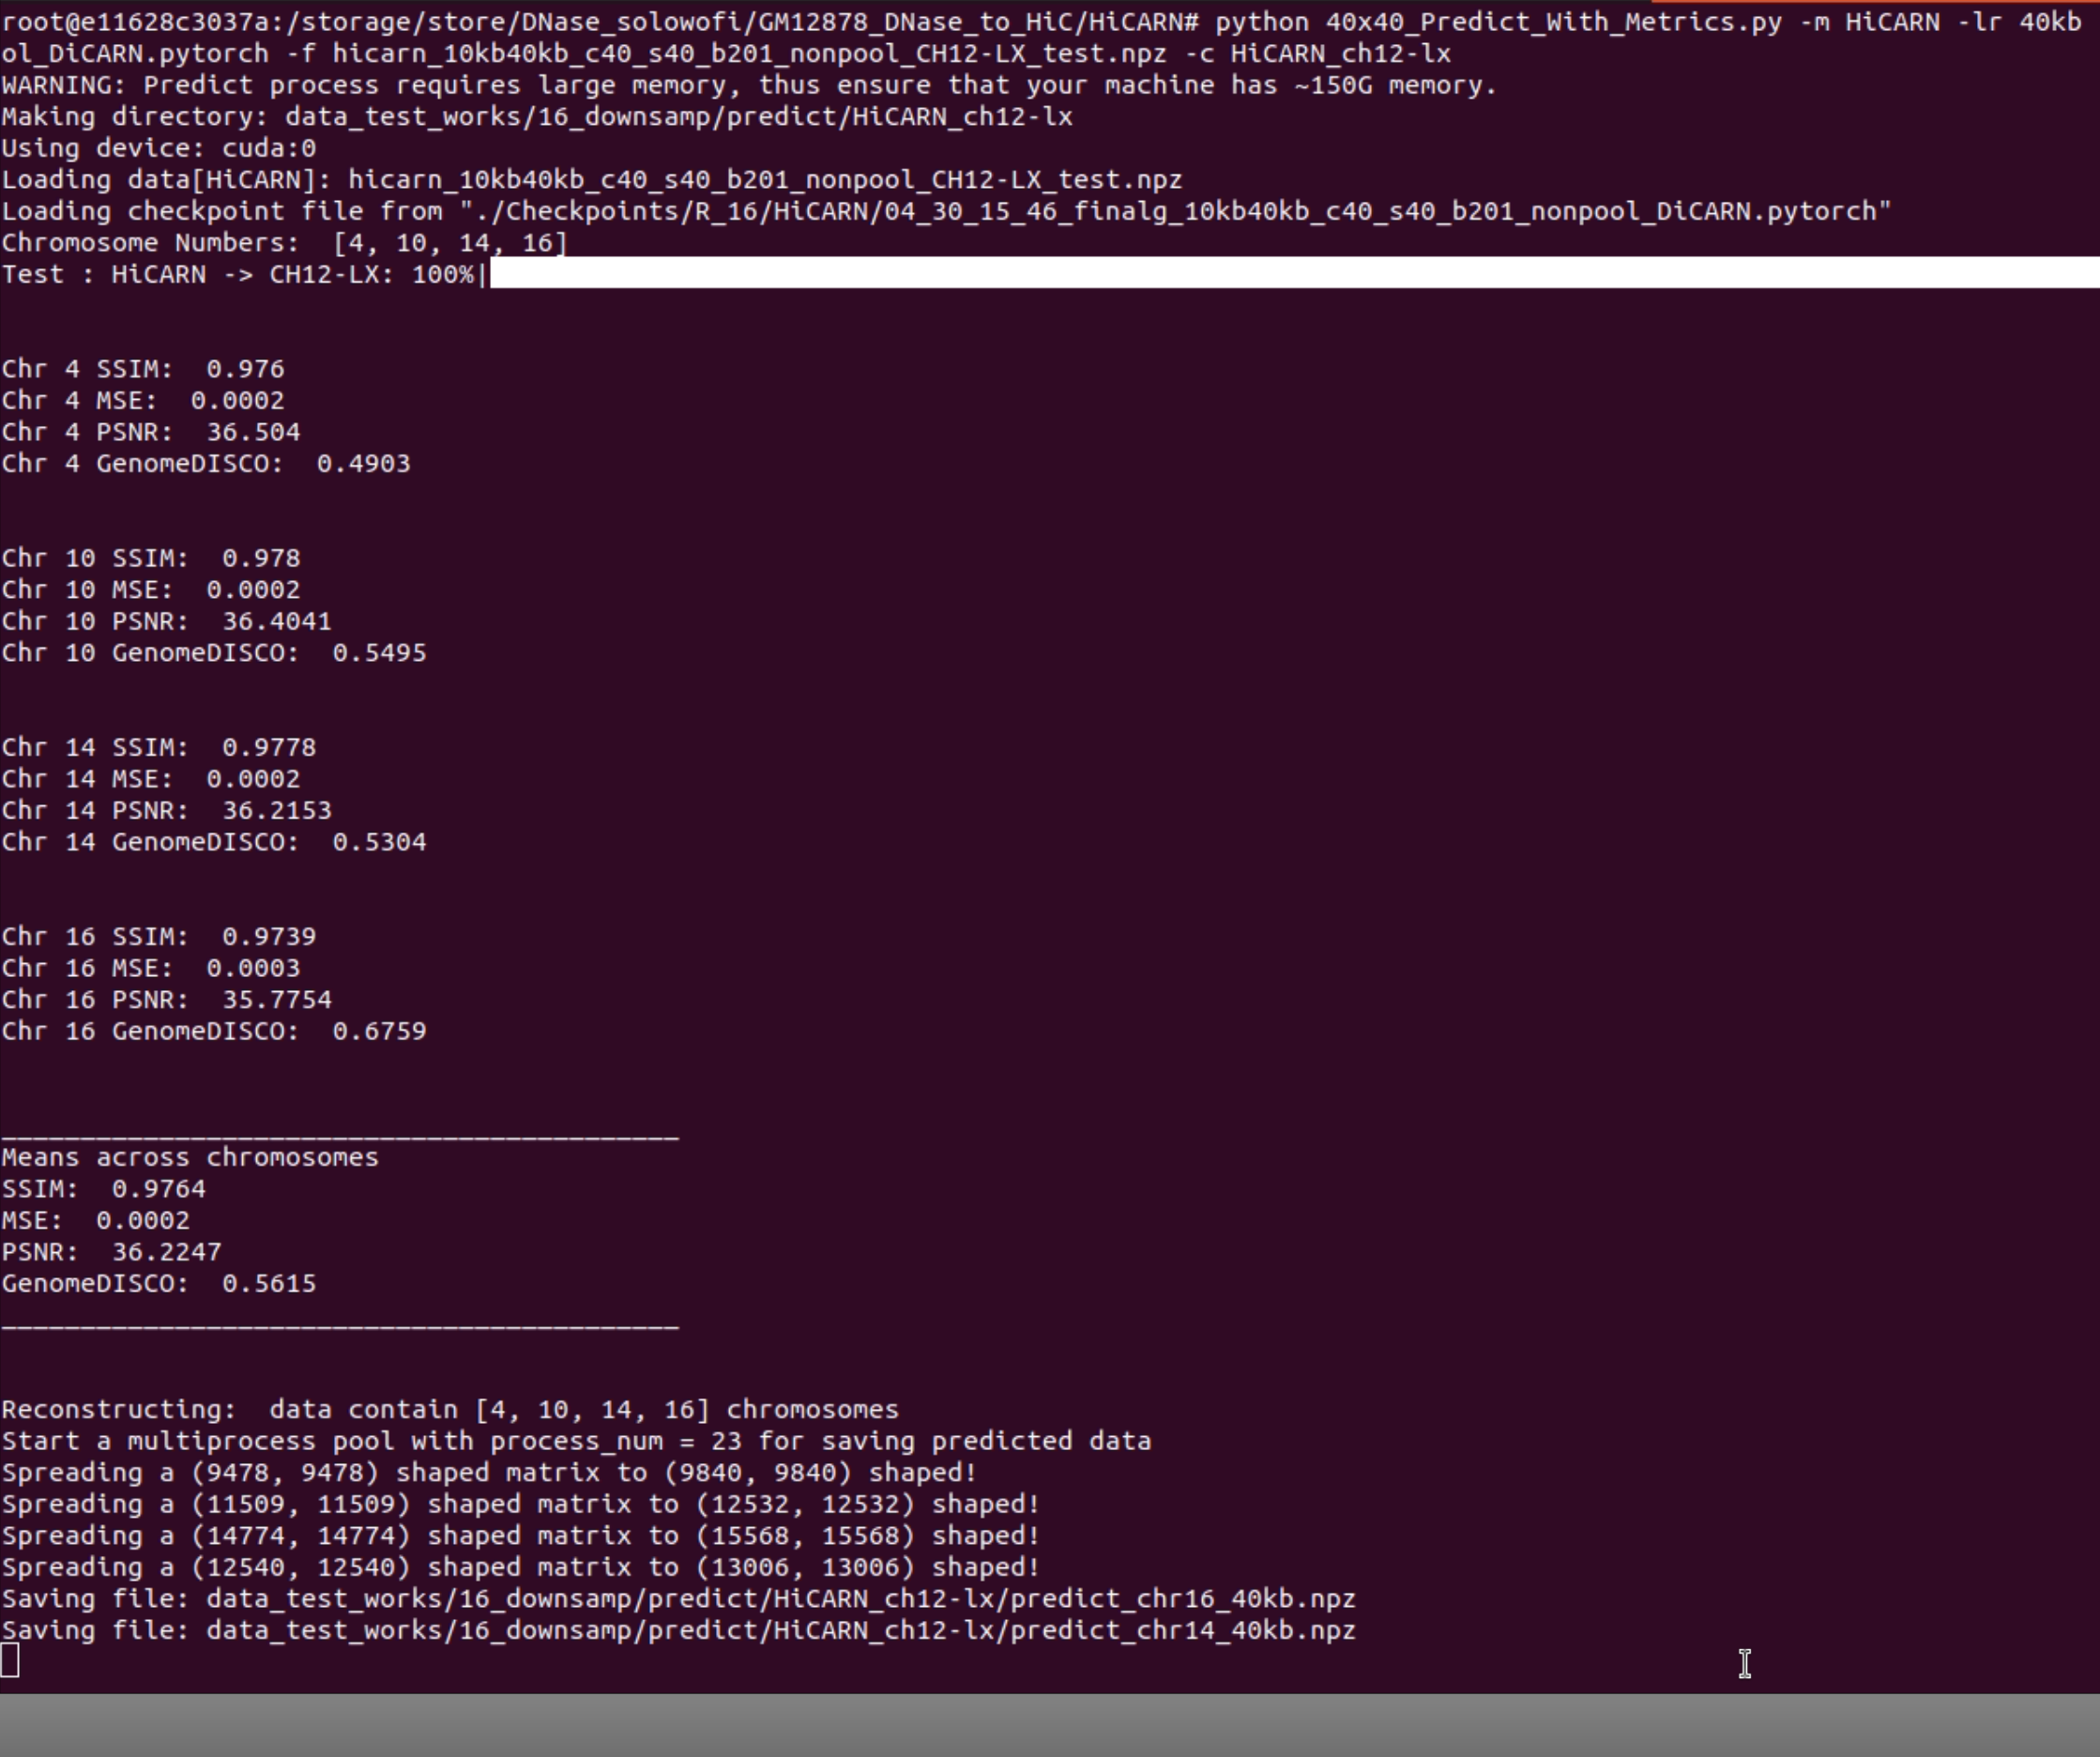
\includegraphics[width=0.5\textwidth]{images/hicarn_screenshot.png}
    \caption{Screenshot of a sample code from the HiCARN Github repository.}
    \label{Samuel}
\end{figure}
\subsection{HiCARN GitHub Exploration Experience}
\begin{itemize}
    \item The ReadMe documentation for the project was detailed enough to follow.
    \item The first challenge I encountered was the state of the dependencies of the codebase, most of which was outdated. I had to find a workable balance between the latest versions of these dependencies and the versions at the time of publication.
    \item The major difficulty encountered was with the default placement of files and subdirectories pulled from the github repo. I had to adjust file and directory interrelationships, as well as some portions of the codebase so that they work as intended.
    \item 
\end{itemize}


\end{document}
